%% A simple template for a lab or course report using the Hagenberg setup
%% based on the standard LaTeX 'report' class
%%% äöüÄÖÜß  <-- no German umlauts here? Use an UTF-8 compatible editor!

%%% Magic comments for setting the correct parameters in compatible IDEs
% !TeX encoding = utf8
% !TeX program = pdflatex 
% !TeX spellcheck = en_US
% !BIB program = biber

\RequirePackage[utf8]{inputenc} % Remove when using lualatex or xelatex!
\RequirePackage{hgbpdfa}        % Creates a PDF/A-2b compliant document

\documentclass[english,smartquotes,apa]{hgbreport}
% Valid options in [..]: 
%    Main language: 'german' (default), 'english'
%    Turn on smart quote handling: 'smartquotes'
%    APA bibliography style: 'apa'
%    Do not create a separate title page: 'notitlepage'
%%%-----------------------------------------------------------------------------

% \renewcommand{\chapter}[1]{} % Disable \chapter command
\graphicspath{{images/}}     % Location of images and graphics
\bibliography{references}    % Biblatex bibliography file (references.bib)
\ExecuteBibliographyOptions{backref=true} % No back references in bibliography

%%%-----------------------------------------------------------------------------
\begin{document}
%%%-----------------------------------------------------------------------------

\author{Tobias Kneidinger, Rafael Hochedlinger}                      % Your name
\title{
	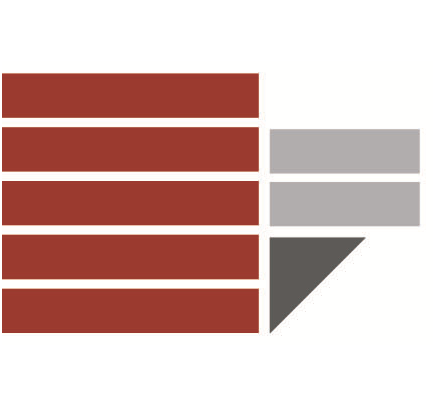
\includegraphics[width=0.3\textwidth]{images/logo-unical.png} \\[1em]
	BDA Report: Neo4j
} % The title of the report
\date{\today}

%%%-----------------------------------------------------------------------------
\maketitle
%%%-----------------------------------------------------------------------------

\tableofcontents

\newpage

%%%-----------------------------------------------------------------------------

\section*{Introduction to Graph Databases}
\addcontentsline{toc}{section}{Introduction to Graph Databases}

Graph Database Management Systems (GDBMS) are a type of NoSQL database which - instead of traditional tables with rows and columns - uses graph structures with nodes, edges, and properties to represent and store data, as seen in \autoref{fig:graph}. This is especially useful for data that is highly interconnected, such as:

\begin{itemize}
	\item Social networks
	\item Recommendation engines
	\item Fraud detection
	\item Network and IT operations
	\item Master data management
	\item Real-time pricing and promotions
	\item Identity and access management
	\item etc\dots
\end{itemize}

\begin{figure}[h]
	\centering
	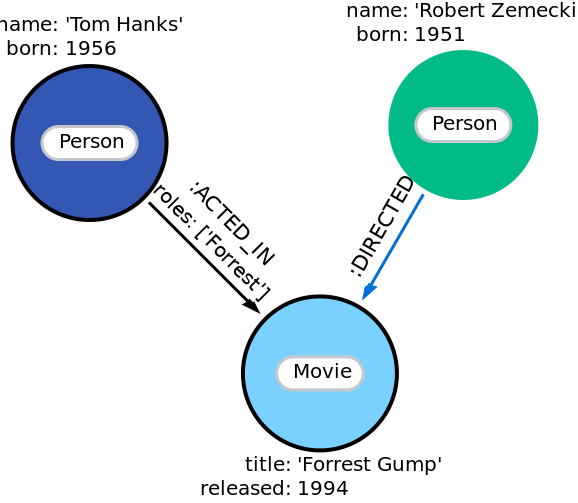
\includegraphics[width=0.5\textwidth]{graphdb.png}
	\caption{Graph Database Structure by \cite{neo4j}}
	\label{fig:graph}
\end{figure}

Graph databases are optimized for traversing and querying graph structures, which makes them very efficient for certain types of queries. As they are NoSQL databases, they are also schema-less and can store data in a flexible way. This makes them also very suitable for machine learning and data science applications, as the data can be stored in a way that is directly usable for the algorithms.

\subsection*{Neo4J}

Neo4J is a popular GDBMS that is used by many companies and organizations. It is developed by Neo Technology and is written in Java, the first version was released in 2007. Neo4J is an open-source database, but there is also a commercial version available with additional features and support. \parencite{neo4j}

It uses the property graph model, which consists of the following elements, as described by \cite{lal2015neo4j}:

\begin{itemize}
	\item \textbf{Nodes}: Entities that represent objects or entities in the graph and can have multiple properties and labels
	\item \textbf{Relationships}: Connect nodes and represent the connections between them, can have a direction and a type and can also have properties
	\item \textbf{Properties}: Key-value pairs that can be attached to nodes and relationships
	\item \textbf{Labels}: Represents the type of a node, can be used to group nodes together
\end{itemize}

The main query language for Neo4J is Cypher, which is a declarative query language that is similar to SQL. These queries can be used to create, read, update, and delete data in the database. The language is more thorouhgly described in the next section.

For data science and machine learning applications, Neo4J also provides the Graph Data Science (GDS) library, which contains a collection of graph algorithms that can be used to analyze and process graph data. This library is also described in more detail in a later section.

%%%-----------------------------------------------------------------------------

\section*{Core Concepts in Neo4j}
\addcontentsline{toc}{section}{Core Concepts in Neo4j}

Neo4j offers a flexible and powerful data model in which the semantic structure of the information is mapped directly in the graph \parencite{robinson2015graph}. The query language of Neo4J Cypher, with which data can be intuitively described as a pattern of nodes and relationships. Cypher queries are more like the visual representation of a graph than the traditional table logic of relational systems, which allows complex connections and paths to be found efficiently.

An essential core aspect of Neo4j is \emph{pattern matching}. Instead of linking several tables via joins, queries in Cypher are described with nodes in round brackets () and relationships in square brackets [], often with arrows to show the direction. This enables a natural form of navigation in the graph. 

The query \autoref{lst:query-employees} finds all persons who are linked to a specific company via a \emph{WORKS\_FOR} relationship. \emph{MATCH} defines the pattern, \emph{WHERE} restricts the results, and \emph{RETURN} returns the desired data. This makes it easy to query even complex graph structures.

\begin{figure}[h]
	\begin{GenericCode}[numbers=none]
	MATCH (p:Person)-[r:WORKS_FOR]->(c:Company)
	WHERE c.name = "Example Company Ltd."
	RETURN p.name, c.name
	\end{GenericCode}
	\caption{Query to find people working for Example Company Ltd.}
	\label{lst:query-employees}
\end{figure}

Neo4j also provides indices and constraints to speed up queries and ensure data integrity. For example, this guarantees unique identifiers and prevents empty values. The flexible modeling makes it possible to introduce new relationships, labels or properties at any time without having to adapt an existing schema. These concepts - from cypher and indices to constraints and flexible schema - are the basis for data analyses in Neo4j.


%%%-----------------------------------------------------------------------------

\section*{Graph Algorithms with GDS}
\addcontentsline{toc}{section}{Graph Algorithms with GDS}

To efficiently analyze and process graph data for data science and machine learning applications, the Graph Data Science (GDS) library can be used. The algorithms in this library are optimized for graph data and can be used to perform various tasks, as described by \cite{neo4j-gds}:

\begin{itemize}
	\item Community detection
	\item Centrality analysis
	\item Link prediction
	\item Similarity analysis
	\item Pathfinding
	\item etc\dots
\end{itemize}

To be able to use conventional neo4j graphs with the GDS library, the graph must be projected into a named graph. This projected graph is a subgraph of the original graph and can be created with the query shown in \autoref{lst:projected-graph}, where 'socialgraph' is the name of the newly projected graph, 'Person' is the node label to project, and 'FRIENDS' is the relationship type to project.

\begin{figure}[h]
	\begin{GenericCode}[numbers=none]
	CALL gds.graph.create('socialgraph', 'Person', 'FRIENDS')
	\end{GenericCode}
	\caption{Projected graph creation}
	\label{lst:projected-graph}
\end{figure}

After the graph has been projected, the GDS algorithms can be used to analyze the graph. In the example shown in \autoref{lst:gds-algorithm}, 
the Louvain algorithm is used to detect communities in the graph. The algorithm is called with the 'socialgraph' as the graph name, the 'Person' node label, and the 'FRIENDS' relationship type. The algorithm yields the nodeId and communityId, which can be used to return the node name and community id. The results are then ordered by the community id.

\begin{figure}[h]
	\begin{GenericCode}[numbers=none]
		CALL gds.louvain.stream('socialgraph')
		YIELD nodeId, communityId
		RETURN gds.util.asNode(nodeId).name AS nodeName, communityId
		ORDER BY communityId;
	\end{GenericCode}
	\caption{GDS algorithm execution}
	\label{lst:gds-algorithm}
\end{figure}

Instead of \lstinline{stream} the algorithm can also be executed with \lstinline{write} to write the results back to the graph. The results can then be used for further analysis or visualization and don't have to be recalcualted every time.

%%%-----------------------------------------------------------------------------

\section*{Performance and Scalability}
\addcontentsline{toc}{section}{Performance and Scalability}

Neo4j uses various techniques to ensure both performance and scalability \parencite{neo4j-operations-manual}.  By using indexes, constraints and intelligent cache strategies, Neo4j can process queries efficiently. In addition, the use of graph algorithms directly in the database makes it possible to perform complex calculations faster without having to export data. The asynchronous processing of queries as well as optimized storage and traversal strategies ensure high performance with growing data volumes.

For the operation of distributed systems, Neo4j supports cluster configurations in which multiple instances of the database work together. This increases both reliability and throughput performance. The causal consistency used here ensures that write and read operations can be traced in a logical sequence, which guarantees consistent data processing, especially in distributed environments.

%%%-----------------------------------------------------------------------------

\section*{Use Cases and Applications}
\addcontentsline{toc}{section}{Use Cases and Applications}

As specified in the introduction, graph databases are especially useful for data that is highly interconnected. This makes them very suitable for a wide range of applications, as described by \cite{neo4j}:

\begin{itemize}
	\item \textbf{Social networks}: To store and analyze user data, relationships, and interactions
	\item \textbf{Recommendation engines}: To provide personalized recommendations based on user behavior
	\item \textbf{Fraud detection}: To detect fraudulent activities and patterns in financial transactions
	\item \textbf{Network and IT operations}: To monitor and analyze network traffic and IT infrastructure
	\item \textbf{Master data management}: To store and manage master data and relationships between entities
	\item \textbf{Real-time pricing and promotions}: To calculate and provide real-time pricing and promotions
	\item \textbf{Identity and access management}: To manage and analyze user identities and access rights
\end{itemize}

The flexibility and scalability of graph databases make them very versatile and suitable for many different use cases, as they can also be combined with other technologies and databases such as relational databases, document databases, or key-value stores.

However, not all use cases are suitable for graph databases. If the data is changing frequently and the relationships don't have to be queried often, another technology - like a relational database - might be the better choice. Also, if the data is not highly interconnected and the queries are simple, a key-value store or document database might be more efficient. 


%%%-----------------------------------------------------------------------------
  
\chapter*{References}
\addcontentsline{toc}{section}{References}
\printbibliography[heading=noheader]


%%%-----------------------------------------------------------------------------
\end{document}
%%%-----------------------------------------------------------------------------
